% !TEX encoding = UTF-8 Unicode
% !TEX program = pdflatex
% !TEX spellcheck = en_US


% In order to correctly compile this document,
% execute the following commands:
% 1. pdflatex
% 2. pdflatex
% 3. pdflatex



\documentclass[amsthm,ebook]{saparticle}

% IF YOU USE PDFLATEX
\usepackage[utf8x]{inputenc}
% if you write in english and in greek
\usepackage{ucs}
\usepackage[greek,english]{babel}
\languageattribute{greek}{polutoniko}

% IF YOU USE XELATEX
%\usepackage{polyglossia}
% if you write in italian
%\setmainlanguage{italian}
% If you want put some ancient greek:
%\setotherlanguage[variant=polytonic]{greek}
%\newfontfamily{\greekfont}[Ligatures=TeX]{Palatino Linotype}

% dummy text (remove in a normal thesis)
% remove if not necessary
\usepackage{siunitx}
%Natbib for bibliography management
\usepackage[authoryear]{natbib}
% custom commands
\newcommand{\bs}{\textbackslash}
\usepackage{xtab}
%%%%%%%%
%TITLE:%
%%%%%%%%

\title{Romans 1 by 1. Documenting a population database for the Roman world}

\author[CLUJ]{Rada Varga\corref{first}}

\address[CLUJ]{Babeș-Bolyai University, Cluj-Napoca}

\cortext[first]{Corresponding author. Email: radavarga@gmail.com}

%\usepackage{longtable}
\begin{document}

\maketitle

\begin{abstract}
 The present article briefly documents the epigraphic division of a developing online population database for the Roman
Empire, accessible at \url{www.romans1by1.com}. The paper presents the motivation of constructing the database and its
envisioned architecture, in relation with the various sources, while emphasizing on the steps and procedures required
in order to transpose epigraphical information into an ancient population database. 
\end{abstract}
\keywords{Epigraphy, middle classes, provincial society, occupational inscriptions, prosopography}



\noindent Romans 1 by 1 database and afferent website were created for filling in an existing gap in the study of Roman-era
population. The database tries to begin answering to the need of properly cataloguing all attested inhabitants of the
Roman Empire. Of course, this is a tremendous task and \url{www.romans1by1.com} is only a first step, circumscribed for now
to a very specific category of sources.


\section{Motivation}


\noindent But why would an ancient population database be essential? Because a digital resource focused on individuals would
reveal linkage possibilities that otherwise elude us, it would finally give us the complete and accurate image of the
Roman attested population and, through codifications, it would open the way towards computer-assisted in-depth analyses
on all relevant aspects imagined (epigraphic patterns, religiosity, migrations, onomastics, occupations, family data,
etc.). A complete, aggregate database will allow a longitudinal (diachronic) view on the attested Roman population from
a certain area and ideally from the whole Empire, while also opening transversal (a section in time) perspectives.

The database in itself would have three components (see below Fig.~\ref{fig:schemadatabase}), following the best practices in the field
(\citet{doi:10.3200/HMTS.37.1.34-38}): the \emph{sources database} (with ``facsimile'' transcription of the sources’ text), the \emph{central database} (the complete, corrected, integrated, standardized and coded form of the sources database) and the \emph{data releases} (destined for on-line usage, allowing easy extraction of data in view of analyses). 

Alongside these components, which actually represent various steps in the data preparation process, a population
database for the Roman Empire should be built on three pillars, which we might call units or divisions of the database:
epigraphic, literary and archaeological, each of them requiring different expertise, different approaches and different
standards for the individual recording forms. In the end, of course, all three types of individual records will have to
be integrated in a central standardized component, whose structure is to be developed by merging the three
aforementioned divisions; consequently, its configuration will ideally take shape only after all three units enjoy a
stable architecture at least in the sources component of the database.

The construction of the database will follow a series of steps imposed by best practices: creating a repository of
sources; introducing, integrating, standardizing, coding and storing the information; enriching and disseminating the
information. The codifications hold an essential part, not only in the individual linkage procedures, but in the
analysing process as well. At the point when the database will comprise enough data, properly recorded and with all
codifications undertaken, the usage of statistical software in order to identify trends and run comparisons over large
scale geographical and administrative units might result in a better than ever understanding of Rome’s
social history.


\begin{figure}[!bp]
\centering
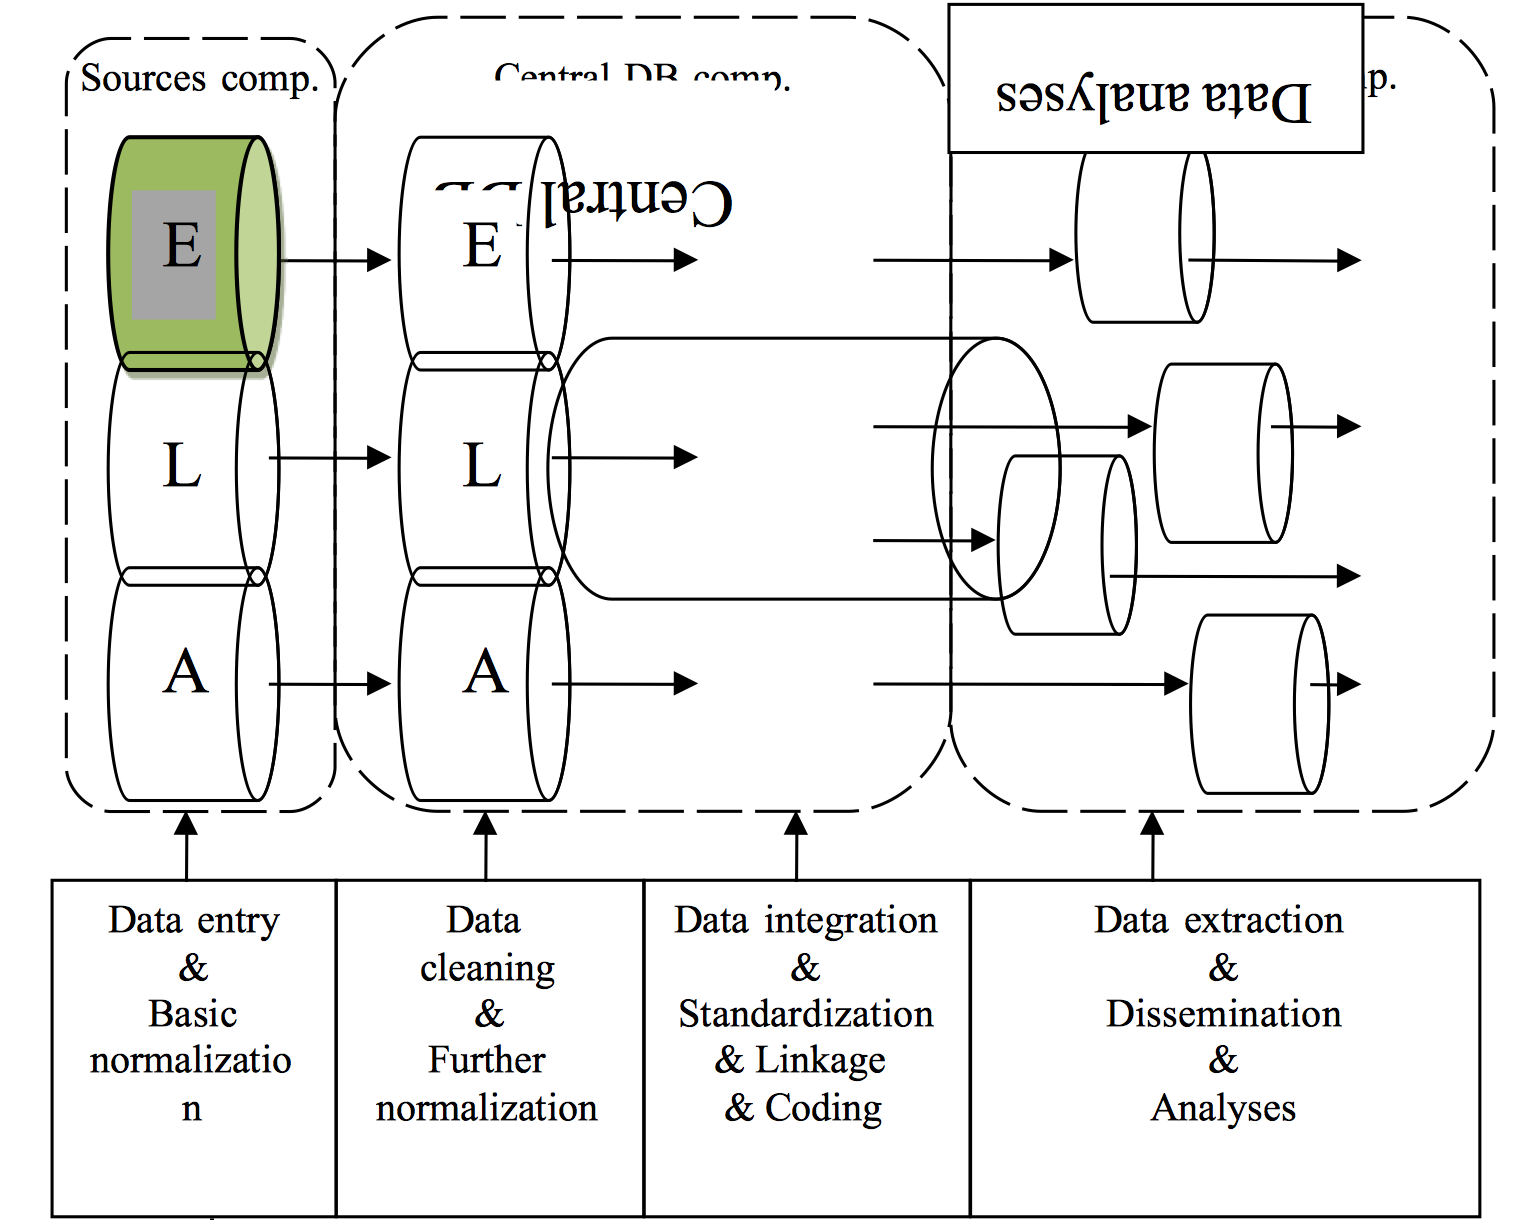
\includegraphics[scale=0.50]{1.png}
\caption{Schema of the database}
\label{fig:schemadatabase}
\end{figure}


\section{The sources}

\noindent Within this theoretical frame, whose amplitude implies a gradual and long-term approach, we have chosen to start by
building the epigraphical division of the database. Thus, we began developing a project on the middle classes of the
Low Danube provinces and their epigraphic attestations. The database created in this context together with the platform
\url{www.romans1by1.com} represent the skeleton of the future population database of the Roman Empire.

For now, we are solely focusing on characters attested epigraphically – thus on inscriptions as sources. As constructing
a metadata suitable for all social and professional categories of the provincial world is very complex, our database is
created for accommodating all information epigraphically provided on members of the provincial middle classes.
Terminologically, we consider all those who manifest themselves epigraphically, without being members of the imperial
or provincial elite, as member of the middle socio-economical layers. Likewise, we have excluded active militaries (but
not their families), as their appurtenance to the army creates their social status.

Regarding the data entry, we are trying to remain faithful to the source and to record, during the first phase, only the
minimum of deduced information (gender, juridical status, ethnicity of the name). At the same time, we operate some
conventional onomastic transcriptions (AEL will be Aelius from the start, etc.). All these basic normalization
procedures are being thoroughly explained and documented in the data entry manual, and the reason why we chose to apply
them is to speed up data standardization, run analyses and publish results on small samples, whose standardization
procedures would otherwise be overwhelmingly time-consuming in relation with the results.

\section{Database architecture}

\noindent The core of the database’s epigraphical division is formed by a table used for recording personal
individual data (labelled \emph{Personal data}), around which the entire network of components needed to ensure proper
information recording is built. However, when starting data entry, one must begin by recording information about the
source in use.

The first table to be filled in is the file of the source – \emph{Inscriptions}. First of all, each inscription gets a source
code, formed of 5 digits and a symbol/acronym of the province’s name (D for Dacia, MS for Moesia Superior, DAL for
Dalmatia, etc.) – so we have, for example 00001MS. The \emph{Inscriptions} table has text fields, as well as value lists.
Then, we have text strings for: \emph{Relevant expressions}, \emph{Stylistic details}, \emph{Atypical features}, \emph{Observations}, \emph{Place of discovery}, \emph{Place of provenience}, \emph{Ancient name provenience}, \emph{Timestamp/Timeframe} and \emph{External links}. Although we are
aware that some of the data (\emph{Timestamp/Timeframe}) could have benefitted from a standardized form, at this point we
opted for vaster possibilities of expression and adaptation. Other information will be filled using value lists, as
standardization is more suited: \emph{Type of inscription}, \emph{Language}, \emph{Material}. For these we will use the Eagle
vocabularies,\footnote{\url{http://www.eagle-network.eu/resources/vocabularies}} because they offer an already
standardized language.

The \emph{Coordinates} table links each inscription with the latitude and longitude of its place of provenience, in order to
place it on a map. 

The \emph{Inscription bibliography} was conceived so that extracting complete or selective bibliographical lists would be
possible. Thus, a normalization table includes all bibliographical titles referred to and from it; through a value
list, one can select the \emph{Bibliography abbreviation}. The exact reference is presented and detailed in the \emph{Details} and
\emph{Comments} text strings. Of course, all data are linked to the \emph{Inscription code}, selected as well from a value list.

Only after properly documenting the source one can access the main and most complex table, \emph{Personal data}, where
basically the individual file of each person is created. At this point, each new entry represents a singular epigraphic
attestation of an individual, and a unique ID is generated, which will help link the respective character throughout
the various components of the database and with other database entries. The person is also manually linked to the
source using a value list of the inscriptions’ codes. In the event of one person being attested in
multiple epigraphs, each attestation will represent a new entry, and it will be assigned a new unique ID, which will be
doubled, during linkage procedures, by a common ID for all instances of the same person. 

The \emph{Personal data} table was built to host a large variety of information offered by epigraphs, and its structure has
proved, up to this day, rather stable. However, if need be, it can always be extended in order to accommodate any new
kind of information. A first set of its variables are name-connected: \emph{Praenomen}, \emph{Nomen}, \emph{Cognomen/Personal name},
\emph{Father/Master} name, \emph{Agnomen}, \emph{Signum}, where each also has a drop-down associated for \emph{Ethnicity} and the \emph{Agnomen} and
\emph{Signum} an \emph{Observations} string. While we believe the possibilities of actually identifying \emph{signa} for members of the
middle classes, during the Principate period, is rather reduced, we opted for facilitating their correct registration,
in case they are discovered. Other data regard \emph{Natione}, \emph{Ethnicity}, \emph{Origo} and \emph{Domus} – if and how they are mentioned in
the inscription. As acknowledged above, some information will be recorded, even if they are deductive and not literally
written in the source: \emph{Gender} and \emph{Juridical status} (though the servile one often is literally recorded). For the
latter, we have opted for a check box, which, if checked, opens all the available possibilities. The rest of the fields
accommodate supplementary information, when and how there is the case: \emph{Occupation}, \emph{Collegium}, \emph{Deities}, \underline{Age} (at death),
\emph{Details of life/death} and \emph{Observations}. 

The \emph{Occupation} field requires some special attention, as it has the \emph{Occupation code} associated with it; as we are trying
to propose a codification of Roman occupations/professions, based on and adapting the HISCO classification
model\footnote{\url{http://historyofwork.iisg.nl/} }. While a raw classification and codification based on HISCO might only
be a slight challenge, finding a theoretical model might prove to be a more elaborated task. What we aim at is
constructing the ``metadata'' for the codification of Roman professions attested on stone and analyse how deep the
classification can realistically go. Much alike other normalization fields present in the sources component of the
database, \emph{Occupation code} was implemented because it helps dealing faster with small and medium size samples (up to
hundreds of people) in view of publishing preliminary results which are vital for dissemination and further financial
support of the project. 

Two important variables, for statistics and working with the data, are \emph{Dedicated by} and \emph{Dedicated for}, which state the
relation of the recorded individual with the epigraph and with other persons mentioned by it. Both appear in the simple
form of check boxes. 

Another particular check box, in need of supplementary explanations, is Later. The database was conceived for attested
civilians from the middle classes, but sometimes they are associated in inscriptions with militaries or representatives
of the elites. In this case, we have to register a minimum of data on the later as well, in order to build a wider
image of the characters that we focus on. When checking \emph{Later}, it opens \emph{Status}, which at its turn opens the following
options in the form of check boxes: \emph{Senator}, \emph{Knight}, \emph{Local magistrate}, \emph{Decurion}, \emph{Imperial priest}, \emph{Imperial slave},
\emph{Imperial freedman}, \emph{Military personnel}. If checked, each of these boxes opens a Details text box; additionally, \emph{Local
magistrate} and \emph{Decurion} open a \emph{City/Town} value list, while \emph{Military personnel}, opens \emph{Rank} and \emph{Unit} value lists. While
elite members and military personnel will at some point be added to the database, for the currently running project
purposes, their social and professional status, together with a minimum of relevant details and relation with the
recorded individuals represent enough information. 
\vspace{20pt}

%\begin{table}[!h]
\tablefirsthead{\hline \textbf{Field label} & \textbf{Field id} & \textbf{Data type} \\ \hline }
\bottomcaption{Metadata of the Personal data table}

%\tablehead{\multicolumn{3}{c}%
%{{\captionsize\bfseries \tablename\ \thetable{} --
%continued from previous page}} \\
%\hline \textbf{Field label} & \textbf{Field id} & \textbf{Data type} \\ \hline }

\tablehead{\hline \textbf{Field label} & \textbf{Field id} & \textbf{Data type} \\ \hline}

\tabletail{\hline \multicolumn{3}{|r|}{{\textit{Continued on next page}}} \\ \hline}
\tablelasttail{\hline}



{\small
\addtolength{\tabcolsep}{-0.5mm}
%\begin{supertabular*}{\textwidth}{p{3.5cm}lp{3cm}}
\begin{xtabular}{|p{.30\textwidth}|p{.30\textwidth}|p{.30\textwidth}|}
%\begin{tabular*}{p{.30\textwidth}p{.29\textwidth}p{.31\textwidth}}
%\toprule
%\textbf{Field label} & \textbf{Field id} & \textbf{Data type}\\\midrule
Praenomen &
rperson\_praenomen &
Text\\ \hline
Ethnicity praenomen &
rperson\_eth\_praen &
Value list\\ \hline
Nomen &
rperson\_nomen &
Text\\ \hline
Ethnicity nomen &
rperson\_eth\_nom &
Value list\\ \hline
Cognomen/Personal name &
rperson\_cognomen &
Text\\ \hline
Ethnicity cognomen/personal name &
rperson\_eth\_cogn &
Value list\\ \hline
Father/Master name &
rperson\_father &
Text\\ \hline
Ethnicity father/master name &
rperson\_eth\_fth &
Value list\\ \hline
Agnomen &
rperson\_agnomen &
Text\\ \hline
Ethnicity agnomen &
rperson\_eth\_agn &
Value list\\ \hline
Observations agnomen &
rperson\_remark\_agn &
Text\\ \hline
Signum &
rperson\_signum &
Text\\ \hline
Ethnicity signum &
rperson\_eth\_sign &
Value list\\ \hline
Observations signum &
rperson\_remark\_sign &
Text\\ \hline
Natione &
rperson\_nation &
Text\\ \hline
Ethnicity &
rperson\_nat\_ethnicity &
Text\\ \hline
Gender &
rperson\_rgender\_id &
Value list\\ \hline
Juridical status &
rperson\_jstatus &
Checkbox. \ Opens checkboxes: 

Citizen, Libertus, Peregrine, Slave 
Veteranus (opens Unit/Rank - valuelists)\\ \hline
Tribus &
rperson\_rtribus\_id &
Text\\ \hline
Origo &
rperson\_origo &
Text\\ \hline
Domus &
rperson\_domus &
Text\\ \hline
Collegium &
rperson\_collegium &
Text\\ \hline
Occupation &
rperson\_occupation &
Text\\ \hline
Occupation code &
rperson\_occ\_code &
Text\\ \hline
Deities &
rperson\_deity &
Text\\ \hline
Age &
rperson\_age &
Text\\ \hline
Details of life/death &
rperson\_death\_details &
Text\\ \hline
Dedicated for & rperson\_dedicated\_for & Checkbox\\ \hline
Inscription code & rperson\_rinscription\_ids & Value list\\ \hline
Later &
rperson\_now\_stat & Checkbox. Opens checkbox:
Status\\ \hline
Status & rperson\_status & Checkbox. Opens checkboxes: 
Senator (opens Details – text),
Knight (opens Details – text) 
Local Magistrate (opens Details – text, City – value list), 
Decurion (opens Details – text, City – value list), 
Imperial priest (opens Details – text), 
Imperial slave (opens Details – text), 
Imperial freedman (opens Details – text), 
Military personnel (opens Details – text, Unit/Rank – value lists)\\ \hline
Observations &
rperson\_observation &
Text\\ \hline
%\bottomrule

\end{xtabular}}
%\caption{This is a wide table where we have used the \texttt{tabular*} environment. Lorem ipsum dolor sit amet, consectetur adipisicing elit, sed do eiusmod tempor incididunt ut labore et dolore magna aliqua.}
%\label{tab:personaldata}
%\end{table}



%\caption{Metadata of the Personal data table}
%\end{supertabular}
%\label{tab:personaldata}
%\end{center}


Based on the personal ID given to each individual, the \emph{Relationship} table will solely name the relationship between
individuals (A to B and B to A), choosing from a drop-down menu. The relationships have been encoded from the start, in
order to make processing quicker; thus first-degree relationships have 10-codes (101-Husband, 102-Wife), second and
third degree relations 20- and respectively 30-codes, non-family relations were given 40- codes and 50-s for the
unspecified/unreadable relations. Male relations were given odd numbers and female ones – even numbers. 

\section{Conclusions}

\noindent \emph{Romans 1 by 1} is a first step towards a comprehensive and exhaustive electronic resource for the attested population of
the Roman Empire. The following normal steps for expanding and enriching the database is elaborating the fitted
metadata for provincial elites and military personnel epigraphically attested.



\section*{Acknowledgement}
This work began being developed during the period of a residential scholarship at the Hardt Fondation, Vandoeuvre. Its
expansion to the area of the whole Latin language Empire is being undertaken with the support of a postdoctoral
fellowship of the Fritz Thyssen Stiftung. Also important was the financial support of a POSDRU scholarship, granted by
the Babeș-Bolyai University.

This work began being developed during the period of a residential scholarship at the Hardt Fondation, Vandoeuvre. Its
expansion to the area of the whole Latin language Empire is being undertaken with the support of a postdoctoral
fellowship of the Fritz Thyssen Stiftung. 

\bibliographystyle{../../sapauth-eng}
\bibliography{../../EAGLE}

\end{document}
